% Esport Language (PaRa) , first experiments
% This is a rapid prototype for planning Pasigraphy Rhapsody (Paszigráfia Rapszódia, PaRa)
%
% con_prel_para.tex
%
% Copyright (C) 2019 Norbert Bátfai, nbatfa@gmail.com, batfai.norbert@inf.unideb.hu
%
%  This program is free software: you can redistribute it and/or modify
%  it under the terms of the GNU General Public License as published by
%  the Free Software Foundation, either version 3 of the License, or
%  (at your option) any later version.
%
%  This program is distributed in the hope that it will be useful,
%  but WITHOUT ANY WARRANTY; without even the implied warranty of
%  MERCHANTABILITY or FITNESS FOR A PARTICULAR PURPOSE.  See the
%  GNU General Public License for more details.
%
%  You should have received a copy of the GNU General Public License
%  along with this program.  If not, see <https://www.gnu.org/licenses/>.
%
% Version history
%
% Initial hack
%
% con_prel_para.tex
% Working title: Construction of the Language of the Esports Culture: A Preliminary Study
%

\documentclass[a4paper]{article}
\usepackage{preamble}

\begin{document}

\title{Az esport kultúra nyelvének megalkotása: egy el\H otanulmány\\Construction of the Language of the Esports Culture: A Preliminary Study}
\author{
	Bátfai Norbert\\
	\texttt{batfai.norbert@inf.unideb.hu}}
\date{
    Információ Technológia Tanszék, Debreceni Egyetem, Magyarország\\
    \today
}

\maketitle

\begin{abstract}
A Paszigráfia Rapszódia \cite{PARAREPO}, vagy röviden PaRa egy olyan mesterséges nyelv kialakítására törekv\H o kezdeményezés, mely lehetővé teszi a homunkulusz és a mesterséges homunkulusz közötti kommunikációt, ergó ez az esport kultúra nyelve \cite{MITEL}. Ebben az el\H otanulmányban megpróbálkozunk ennek a nyelvnek a megalkotásával.
\end{abstract}

{
\selectlanguage{english}
\begin{abstract}
The Pasigraphy Rhapsody \cite{PARAREPO}, or shortly PaRa (from it's Hungarian name Paszigr\'afia Rapsz\'odia) is an initiative to develop an artificial language that is intended to allow communication between the Homunculus and the Artificial Homunculus, ergo, it is the language of the esport culture \cite{MITEL}.
In this preliminary study, we have tried to construct this language.
\end{abstract}
}

{
\selectlanguage{magyar}

\section{Bevezetés}

A PaRa vizualizációjának \cite{VISPARA} alapját az SMNIST képek \cite{SMNIST} képezik, ahol a képeken lév\H o pöttyök számosságát kell meghatározni. Ám meg kell jegyezzük, hogy a PaRa esetében nem a számosság, hanem a pöttyök pontos helyzete a meghatározó.
}

{
\selectlanguage{english}
\section{Introduction}

The intuitive base of visualization of PaRa \cite{VISPARA} comes from SMNIST images \cite{SMNIST}, where the numerosity of dots must be recognized in images. But it should be noticed that in the case of PaRa the numerosity does not matter but the exact position of the dots.
}

\subsection{Els\H o próbálkozások}

\begin{itemize}
\item[NP] Legyen adott egy természetes nyelv\H u $s$ mondat.
\item[FOL] Próbálkozzunk meg $s$ els\H orend\H u logikai formalizálásával,
nevezzünk ezt $F(s)$-nek ami a Paszigráfia Rapszódia el\H onyelvének mondata lesz. Ez azt jelenti, hogy $s$ jelentését meg kell próbálnunk kifejezni a PaRa el\H onyelvén. Itt arra rá kell mutatnunk, hogy ez a folyamat bem algoritmizálható. Ezt a lépést mindig a humán játékos hajtja végre.
\item[TILE] Majd rajzoljuk át $F(s)$-t a PaRa csempéz\H o rácsba.
\item[NUM] Convert cells of the tiling grid into unique numbers.
\item[SMNIST] Convert these unique numbers into SMNIST codes.
\item[NDIM] Végül egy n dimenziós hiperkocka formájában vizualizáljuk az eredményt.
\end{itemize}

\subsection{First Attempts}

\begin{itemize}
\item[NP] Let be given a natural language sentence $s$.
\item[FOL] Try to find a first order logic formalization for $s$. Let's called it $F(s)$ that is a sentence of the proto-language of Pasigraphy Rhapsody.
This means that the meaning of $s$ must be tried to express in the proto-language of PaRa.
It should be noticed that this process cannot be algorithmized.
This step is always performed by the human player. But the following steps labelled by TILE, NUM, SMNIST and NDIM can be fully automated.
\item[TILE] Then draw $F(s)$ in the form of PaRa tiling grid.
\item[NUM] Convert cells of the tiling grid into unique numbers.
\item[SMNIST] Convert these unique numbers into SMNIST codes.
\item[NDIM] Finally visualize the results as an n-dimensional hypercube.
\end{itemize}

\begin{example}
\begin{center}
\begin{tabular}{|>{\centering\arraybackslash}m{4cm}|m{4cm}|>{\centering\arraybackslash}m{4cm}|}\hline
\centering
\textbf{English} & \textbf{PaRa 2D} & \textbf{PaRa 3D}  \\
\hline
Mice hate cats. &
\begin{tikzpicture}[thick,scale=.6, every node/.style={scale=.6}]
\prelparaIID{"4:2:1:1:0:3:2:1:0:2:0:2:1:1:0:3:3:0:2:0:1:1:0"}
\end{tikzpicture}
\newline
\begin{tikzpicture}[thick,scale=.6, every node/.style={scale=.6}]
\prelparaIID{"6:1:0:2:2:0:1:1:1:3:2:1:0:2:0:2:1:1:1:2:3:0:1:1:0:1:1:3:3:0:1:0:2:1:0"}
\end{tikzpicture}
\newline
\begin{tikzpicture}[thick,scale=.6, every node/.style={scale=.6}]
\prelparaIID{"5:1:0:2:2:0:0:0:1:3:1:0:1:3:2:1:0:2:0:3:3:0:2:0:1:1:0"}
\end{tikzpicture}
&
\begin{tikzpicture}[thick,scale=.6, every node/.style={scale=.6}]
\prelparaIIID{1}{"3:2:1:1:0:3:2:1:0:2:0:2:1:1:0:1:0:2:2:0:1:1:1:3:2:1:0:2:0:1:0:2:2:0:0:0:1:3:1:0:1"}
\end{tikzpicture}
 \\\hline
\end{tabular}
\end{center}
\end{example}


\subsubsection{The syntax of the proto-language of Pasigraphy Rhapsody}

Here we use the notations of Albert Drag\'alin  \cite{ALBERT} and the book \cite{RusselNorvig} together.

\paragraph{Types}
\begin{bnf}
\bnfprod{Index} {\bnfts{\stick} \bnfsp \bnfpn{Index}  \bnfor \bnfts{\stick}}\\
\bnfprod{Srt} {\bnfpn{Index}}
\end{bnf}

\paragraph{Variables}
\begin{bnf}
\bnfprod{Variable} {\bnfts{(}\bnfpn{Srt}\bnfts{.}\bnfpn{Index}\bnfts{)}}
\end{bnf}

\paragraph{Constants}
\begin{bnf}
\bnfprod{Cnst} {\bnfts{(C.}\bnfpn{Srt}\bnfts{.}\bnfpn{Index}\bnfts{)}}
\end{bnf}

\paragraph{Functions}
\begin{bnf}
\bnfprod{Fn} {\bnfts{(F.}\bnfpn{Index}\bnfpn{ParamList}\bnfts{)}}
\end{bnf}
\begin{bnf}
\bnfprod{ParamList} {\bnfes \bnfor \bnfts{(}\bnfpn{ParamListBuilder}\bnfts{)}}
\end{bnf}
\begin{bnf}
\bnfprod{ParamListBuilder} {\bnfpn{Term} \bnfor \bnfpn{Term}\bnfts{,} \bnfpn{ParamListBuilder}}
\end{bnf}

\paragraph{Predicates}
\begin{bnf}
\bnfprod{Pr} {\bnfts{(P.}\bnfpn{Index}\bnfpn{ParamList}\bnfts{)}}
\end{bnf}

\paragraph{Terms}
\begin{bnf}
\bnfprod{Term} {\bnfpn{Variable} \bnfor \bnfpn{Cnst} \bnfor \bnfpn{Fn}}
\end{bnf}

\paragraph{Atomic Formulas}
\begin{bnf}
\bnfprod{Atomic Formula} {\bnfpn{Pr}}
\end{bnf}

\paragraph{Formulas}
\begin{bnf}
	\bnfprod{Formula} {\bnfpn{Atomic Formula} \bnfor \bnfts{\neg}\bnfpn{Formula} \bnfor}\\
	\bnfmore{\bnfpn{Formula}\bnfpn{Connective}\bnfpn{Formula} \bnfor}\\
	\bnfmore{\bnfpn{Quantifier}\bnfpn{Variable}\bnfpn{Formula}}
\end{bnf}

\paragraph{Logical Connectives}
\begin{bnf}
\bnfprod{Connective} {\bnfts{\wedge} \bnfor \bnfts{\vee} \bnfor \bnfts{\supset} }
\end{bnf}

\paragraph{Quantifiers}
\begin{bnf}
\bnfprod{Quantifier} {\bnfts{\exists} \bnfor \bnfts{\forall} }
\end{bnf}

{
\selectlanguage{magyar}

\begin{pelda}
Formalizáljuk a következő természetes nyelvi kijelentést!
$$
\text{Az egerek utálják a macskákat.}
$$
$$\forall \text{Állat.}x \forall \text{Állat.}y ( \text{P.Egér}(x) \wedge \text{P.Macska}(y)  \supset \text{P.Utál}(x, y))$$
Kicsit jobban megfeleltetve a grammatikának azt írnánk, hogy
$$\forall (1.1) \forall (1.2) (
(P.1 (1.1)) \wedge (P.2 (1.2))
\supset
(P.3(1.1, 1.2))
)$$
szóval mindent szépen számozgatunk, itt például minden változót és prédikátumot külön, a felbukkanásuk rendjében. Ha ez a mondat volt a "Helló, Világ!"\footnote{Tehát az els\H o formalizált mondatunk.} mondatunk, akkor most éppen ezeket a táblázatokat kell karban tartanunk:

\begin{center}
\begin{tabular}{ll}
\centering
\textbf{Típus} & \textbf{Prédikátum}\\
Állat=1& Egér=1\\
& Macska=2\\
& Utál=3
\end{tabular}
\end{center}

Méginkább közelítve a grammatikához pedig ezt írnánk
$$\forall (\stick . \stick) \forall (\stick . \stick \ \stick) (
(P . \stick (\stick . \stick)) \wedge (P . \stick \ \stick (\stick . \stick \ \stick))
\supset
(P . \stick \ \stick \ \stick(\stick . \stick, \stick . \stick \ \stick))
)$$
ami még mindig elég pongyola, de pontosabbá már a grammmatikával együttesen
történ\H o pontosítással tehetnénk (például a zárójelezés tekintetében), de nem tesszük, mert a formalizálásoknál úgyis maradunk az els\H o formánál, s számozni is egészen máshogy fogunk. Tehát a grammatikával mindössze annyit rögzítettünk, hogy elvben megszámlálhatóan végtelen sok típust, változót, kontanst, prédikátumot és függvényt akarunk felhasználni.
\end{pelda}
}

\subsubsection{The PaRa Tiling Language}

A zárójelezést a behúzással váltjuk ki.

\begin{pelda}
\begin{center}
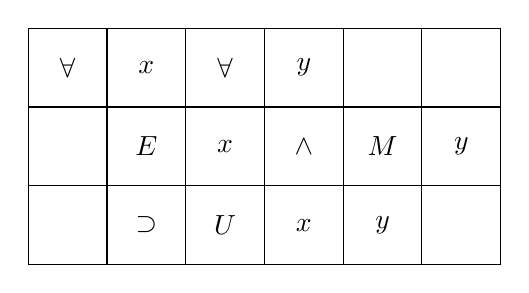
\begin{tikzpicture}
\foreach \x in {1,2,...,6}
\foreach \y in {3,...,1}
{
\draw (\x,3-\y) +(-.5,-.5) rectangle +(.5,.5);
%\draw (\x,9-\y) node{\x,\y};
}
\draw (1,3-1) node{$\forall$};
\draw (2,3-1) node{$x$};
\draw (3,3-1) node{$\forall$};
\draw (4,3-1) node{$y$};

\draw (2,3-2) node{$E$};
\draw (3,3-2) node{$x$};
\draw (4,3-2) node{$\wedge$};
\draw (5,3-2) node{$M$};
\draw (6,3-2) node{$y$};

\draw (2,3-3) node{$\supset$};
\draw (3,3-3) node{$U$};
\draw (4,3-3) node{$x$};
\draw (5,3-3) node{$y$};
\end{tikzpicture}
\end{center}

Kicsit kevésbé leegyszer\H usítve.

\begin{center}
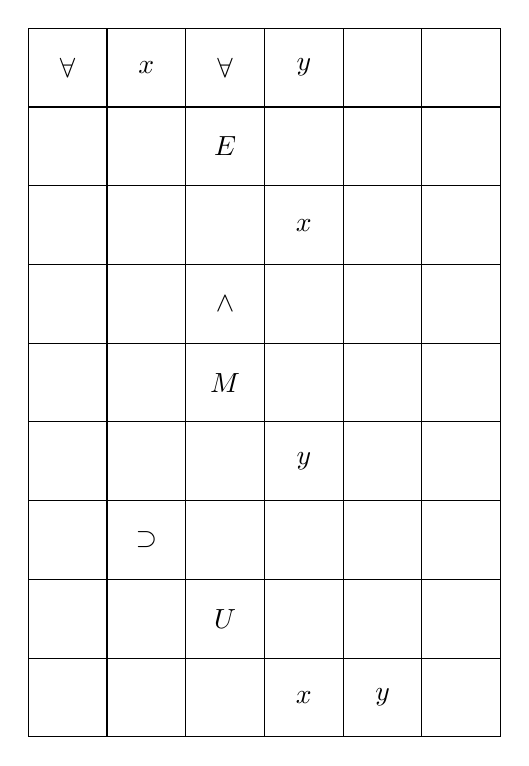
\begin{tikzpicture}
\foreach \x in {1,2,...,6}
\foreach \y in {9,...,1}
{
\draw (\x,9-\y) +(-.5,-.5) rectangle +(.5,.5);
%\draw (\x,9-\y) node{\x,\y};
}
\draw (1,9-1) node{$\forall$};
\draw (2,9-1) node{$x$};
\draw (3,9-1) node{$\forall$};
\draw (4,9-1) node{$y$};

\draw (3,9-2) node{$E$};
\draw (4,9-3) node{$x$};
\draw (3,9-4) node{$\wedge$};
\draw (3,9-5) node{$M$};
\draw (4,9-6) node{$y$};

\draw (2,9-7) node{$\supset$};
\draw (3,9-8) node{$U$};
\draw (4,9-9) node{$x$};
\draw (5,9-9) node{$y$};
\end{tikzpicture}
\end{center}
\end{pelda}

Persze ki kellene írnunk a grammatika terminális \textquote{karácsonyfáit} (például a típusokat és a sorszámot elválasztó pontot, vagy a predikátumokat bevezet\H o P bet\H ut stb.), de nem ezt fogjuk tenni, hanem bevezetünk egy egységes számozási rendszert.

\subsubsection{The PaRa Numeration System}

\begin{center}
\begin{tabular}{|c|c|}\hline
\centering
\textbf{Terminális bet\H u} & \textbf{PaRa számkód}   \\
\hline
$\exists$ & 1 \\
\hline
$\forall$ & 2 \\
\hline
$\neg$ & 3 \\
\hline
$\wedge$ & 4 \\
\hline
$\vee$ & 5 \\
\hline
$\supset$ & 6 \\\hline
\end{tabular}
\end{center}
Maradt még megszámlálhatóan végtelen prédikátum, függvény és típus nevünk, illetve minden megszámlálható típuson belül ugyancsak megszámlálható konstans és változó nevünk. Ezeket is könnyen számba vehetjük például Péter Rózsa könyvéb\H ol a transzfinit indukció bevezetése kapcsán említett, a természetes számokat megszámlálható sok diszjunk részhamazra bontását bemutató példájával, azaz

\begin{itemize}
\item A $PaRa_\text{text}=\{7, 9, 11, 13, 15, 17, \dots \}$ halmaz, avagy a páratlan számokból kiszedve a terminális bet\H uk kódjait, jelöli a már el\H oállított PaRa szövegek indexeit.
Minden előállított PaRa szöveget (például egy PaRa csempézési mátrixot, vagy a formalizált PaRa előnyelvi formulákat) megjegyzünk egy listában, ennek indexét adja a páratlan szám eképpen: $\frac{\text{páratlan szám} - 1}{2}-2$.
\item A $PaRa_\text{pred}=\{10, 14, 18, 22, 26, \dots \}$ halmaz, avagy a kett\H onek csak az els\H o hatványával oszthatóak (megint csak kiszedve a terminálisok) jelölik a PaRa prédikátumokat.
\item A $PaRa_\text{fn}=\{12, 20, 28, 36, 44, \dots \}$ halmaz, avagy a kett\H onek legfeljebb csak a második hatványával oszthatóak (ugyancsak kiszedve a terminálisok) jelölik a PaRa függvényeket.
\item A $PaRa_\text{srt}=\{8, 24, 40, 56, 72, \dots \}$ halmaz, avagy a kett\H onek legfeljebb csak a harmadik hatványával oszthatóak jelölik a PaRa típusokat.
\item A $PaRa_{c_1}=\{16, 48, 80, 112, 144, \dots \}$ halmaz, avagy a kett\H onek legfeljebb csak a negyedik hatványával oszthatóak jelölik a PaRa els\H o típusának végtelen sok konstansát.
\item A $PaRa_{v_1}=\{32, 96, 160, 224, 288, \dots \}$ halmaz, avagy a kett\H onek legfeljebb csak a ötödik hatványával oszthatóak jelölik a PaRa els\H o típusának végtelen sok változóját.
\item \dots
\item A $PaRa_{c_n}=\{2^{2n+2}, 2^{2n+2}+2^{2n+3}, 2^{2n+2}+2*2^{2n+3},  2^{2n+2}+3*2^{2n+3}, \dots \}$ halmaz, avagy a kett\H onek legfeljebb csak az $2n+2$. hatványával oszthatóak jelölik a PaRa $n$. típusának végtelen sok konstansát.
\item A $PaRa_{v_n}=\{2^{2n+3}, 2^{2n+3}+2^{2n+4}, 2^{2n+3}+2*2^{2n+4},  2^{2n+3}+3*2^{2n+4}, \dots \}$ halmaz, avagy a kett\H onek legfeljebb csak az $2n+3$. hatványával oszthatóak jelölik a PaRa $n$. típusának végtelen sok változóját.
\item \dots
\end{itemize}



\begin{pelda}
\begin{center}
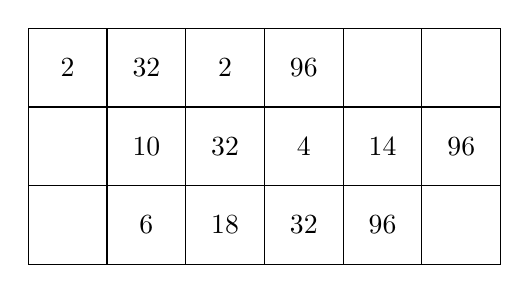
\begin{tikzpicture}
\foreach \x in {1,2,...,6}
\foreach \y in {3,...,1}
{
\draw (\x,3-\y) +(-.5,-.5) rectangle +(.5,.5);
}
\draw (1,3-1) node{$2$};
\draw (2,3-1) node{$32$};
\draw (3,3-1) node{$2$};
\draw (4,3-1) node{$96$};

\draw (2,3-2) node{$10$};
\draw (3,3-2) node{$32$};
\draw (4,3-2) node{$4$};
\draw (5,3-2) node{$14$};
\draw (6,3-2) node{$96$};

\draw (2,3-3) node{$6$};
\draw (3,3-3) node{$18$};
\draw (4,3-3) node{$32$};
\draw (5,3-3) node{$96$};

\end{tikzpicture}
\end{center}

\begin{center}
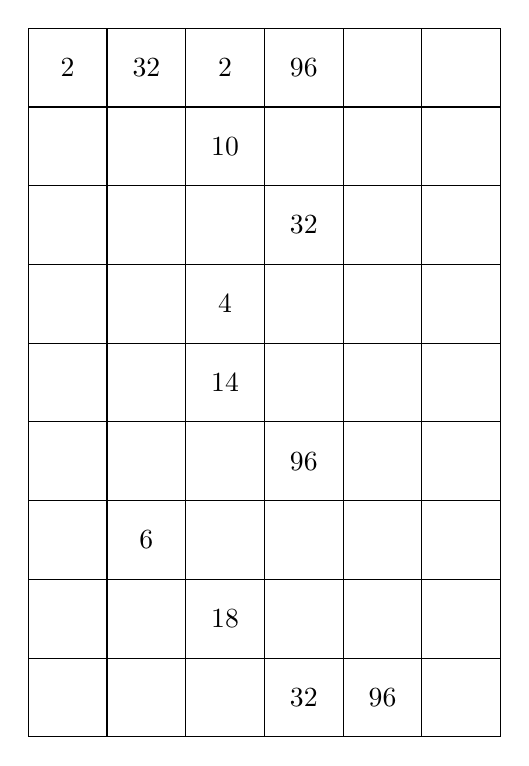
\begin{tikzpicture}
\foreach \x in {1,2,...,6}
\foreach \y in {9,...,1}
{
\draw (\x,9-\y) +(-.5,-.5) rectangle +(.5,.5);
}
\draw (1,9-1) node{$2$};
\draw (2,9-1) node{$32$};
\draw (3,9-1) node{$2$};
\draw (4,9-1) node{$96$};

\draw (3,9-2) node{$10$};
\draw (4,9-3) node{$32$};
\draw (3,9-4) node{$4$};
\draw (3,9-5) node{$14$};
\draw (4,9-6) node{$96$};

\draw (2,9-7) node{$6$};
\draw (3,9-8) node{$18$};
\draw (4,9-9) node{$32$};
\draw (5,9-9) node{$96$};
\end{tikzpicture}
\end{center}
\end{pelda}

\subsubsection{SMNIST codes}

\begin{lstlisting}[breaklines]
n: 4 k: 1 index: 1 1: (0,0)
n: 4 k: 1 index: 2 1: (1,0)
n: 4 k: 1 index: 3 1: (0,1)
n: 4 k: 1 index: 4 1: (1,1)
*****
n: 4 k: 2 index: 5 1: (0,0) 2: (1,0)
n: 4 k: 2 index: 6 1: (0,0) 2: (0,1)
n: 4 k: 2 index: 7 1: (0,0) 2: (1,1)
n: 4 k: 2 index: 8 1: (1,0) 2: (0,1)
n: 4 k: 2 index: 9 1: (1,0) 2: (1,1)
n: 4 k: 2 index: 10 1: (0,1) 2: (1,1)
*****
n: 4 k: 3 index: 11 1: (0,0) 2: (1,0) 3: (0,1)
n: 4 k: 3 index: 12 1: (0,0) 2: (1,0) 3: (1,1)
n: 4 k: 3 index: 13 1: (0,0) 2: (0,1) 3: (1,1)
n: 4 k: 3 index: 14 1: (1,0) 2: (0,1) 3: (1,1)
*****
n: 9 k: 1 index: 15 1: (0,0)
n: 9 k: 1 index: 16 1: (1,0)
n: 9 k: 1 index: 17 1: (2,0)
n: 9 k: 1 index: 18 1: (0,1)
n: 9 k: 1 index: 19 1: (1,1)
n: 9 k: 1 index: 20 1: (2,1)
n: 9 k: 1 index: 21 1: (0,2)
n: 9 k: 1 index: 22 1: (1,2)
n: 9 k: 1 index: 23 1: (2,2)
*****
n: 9 k: 2 index: 24 1: (0,0) 2: (1,0)
n: 9 k: 2 index: 25 1: (0,0) 2: (2,0)
n: 9 k: 2 index: 26 1: (0,0) 2: (0,1)
n: 9 k: 2 index: 27 1: (0,0) 2: (1,1)
n: 9 k: 2 index: 28 1: (0,0) 2: (2,1)
n: 9 k: 2 index: 29 1: (0,0) 2: (0,2)
n: 9 k: 2 index: 30 1: (0,0) 2: (1,2)
n: 9 k: 2 index: 31 1: (0,0) 2: (2,2)
n: 9 k: 2 index: 32 1: (1,0) 2: (2,0)
n: 9 k: 2 index: 33 1: (1,0) 2: (0,1)
n: 9 k: 2 index: 34 1: (1,0) 2: (1,1)
n: 9 k: 2 index: 35 1: (1,0) 2: (2,1)
n: 9 k: 2 index: 36 1: (1,0) 2: (0,2)
n: 9 k: 2 index: 37 1: (1,0) 2: (1,2)
n: 9 k: 2 index: 38 1: (1,0) 2: (2,2)
n: 9 k: 2 index: 39 1: (2,0) 2: (0,1)
n: 9 k: 2 index: 40 1: (2,0) 2: (1,1)
n: 9 k: 2 index: 41 1: (2,0) 2: (2,1)
n: 9 k: 2 index: 42 1: (2,0) 2: (0,2)
n: 9 k: 2 index: 43 1: (2,0) 2: (1,2)
n: 9 k: 2 index: 44 1: (2,0) 2: (2,2)
n: 9 k: 2 index: 45 1: (0,1) 2: (1,1)
n: 9 k: 2 index: 46 1: (0,1) 2: (2,1)
n: 9 k: 2 index: 47 1: (0,1) 2: (0,2)
n: 9 k: 2 index: 48 1: (0,1) 2: (1,2)
n: 9 k: 2 index: 49 1: (0,1) 2: (2,2)
n: 9 k: 2 index: 50 1: (1,1) 2: (2,1)
n: 9 k: 2 index: 51 1: (1,1) 2: (0,2)
n: 9 k: 2 index: 52 1: (1,1) 2: (1,2)
n: 9 k: 2 index: 53 1: (1,1) 2: (2,2)
n: 9 k: 2 index: 54 1: (2,1) 2: (0,2)
n: 9 k: 2 index: 55 1: (2,1) 2: (1,2)
n: 9 k: 2 index: 56 1: (2,1) 2: (2,2)
n: 9 k: 2 index: 57 1: (0,2) 2: (1,2)
n: 9 k: 2 index: 58 1: (0,2) 2: (2,2)
n: 9 k: 2 index: 59 1: (1,2) 2: (2,2)
*****
n: 9 k: 3 index: 60 1: (0,0) 2: (1,0) 3: (2,0)
n: 9 k: 3 index: 61 1: (0,0) 2: (1,0) 3: (0,1)
n: 9 k: 3 index: 62 1: (0,0) 2: (1,0) 3: (1,1)
n: 9 k: 3 index: 63 1: (0,0) 2: (1,0) 3: (2,1)
n: 9 k: 3 index: 64 1: (0,0) 2: (1,0) 3: (0,2)
n: 9 k: 3 index: 65 1: (0,0) 2: (1,0) 3: (1,2)
n: 9 k: 3 index: 66 1: (0,0) 2: (1,0) 3: (2,2)
n: 9 k: 3 index: 67 1: (0,0) 2: (2,0) 3: (0,1)
n: 9 k: 3 index: 68 1: (0,0) 2: (2,0) 3: (1,1)
n: 9 k: 3 index: 69 1: (0,0) 2: (2,0) 3: (2,1)
n: 9 k: 3 index: 70 1: (0,0) 2: (2,0) 3: (0,2)
n: 9 k: 3 index: 71 1: (0,0) 2: (2,0) 3: (1,2)
n: 9 k: 3 index: 72 1: (0,0) 2: (2,0) 3: (2,2)
n: 9 k: 3 index: 73 1: (0,0) 2: (0,1) 3: (1,1)
n: 9 k: 3 index: 74 1: (0,0) 2: (0,1) 3: (2,1)
n: 9 k: 3 index: 75 1: (0,0) 2: (0,1) 3: (0,2)
n: 9 k: 3 index: 76 1: (0,0) 2: (0,1) 3: (1,2)
n: 9 k: 3 index: 77 1: (0,0) 2: (0,1) 3: (2,2)
n: 9 k: 3 index: 78 1: (0,0) 2: (1,1) 3: (2,1)
n: 9 k: 3 index: 79 1: (0,0) 2: (1,1) 3: (0,2)
n: 9 k: 3 index: 80 1: (0,0) 2: (1,1) 3: (1,2)
n: 9 k: 3 index: 81 1: (0,0) 2: (1,1) 3: (2,2)
n: 9 k: 3 index: 82 1: (0,0) 2: (2,1) 3: (0,2)
n: 9 k: 3 index: 83 1: (0,0) 2: (2,1) 3: (1,2)
n: 9 k: 3 index: 84 1: (0,0) 2: (2,1) 3: (2,2)
n: 9 k: 3 index: 85 1: (0,0) 2: (0,2) 3: (1,2)
n: 9 k: 3 index: 86 1: (0,0) 2: (0,2) 3: (2,2)
n: 9 k: 3 index: 87 1: (0,0) 2: (1,2) 3: (2,2)
n: 9 k: 3 index: 88 1: (1,0) 2: (2,0) 3: (0,1)
n: 9 k: 3 index: 89 1: (1,0) 2: (2,0) 3: (1,1)
n: 9 k: 3 index: 90 1: (1,0) 2: (2,0) 3: (2,1)
n: 9 k: 3 index: 91 1: (1,0) 2: (2,0) 3: (0,2)
n: 9 k: 3 index: 92 1: (1,0) 2: (2,0) 3: (1,2)
n: 9 k: 3 index: 93 1: (1,0) 2: (2,0) 3: (2,2)
n: 9 k: 3 index: 94 1: (1,0) 2: (0,1) 3: (1,1)
n: 9 k: 3 index: 95 1: (1,0) 2: (0,1) 3: (2,1)
n: 9 k: 3 index: 96 1: (1,0) 2: (0,1) 3: (0,2)
n: 9 k: 3 index: 97 1: (1,0) 2: (0,1) 3: (1,2)
n: 9 k: 3 index: 98 1: (1,0) 2: (0,1) 3: (2,2)
n: 9 k: 3 index: 99 1: (1,0) 2: (1,1) 3: (2,1)
n: 9 k: 3 index: 100 1: (1,0) 2: (1,1) 3: (0,2)
n: 9 k: 3 index: 101 1: (1,0) 2: (1,1) 3: (1,2)
n: 9 k: 3 index: 102 1: (1,0) 2: (1,1) 3: (2,2)
n: 9 k: 3 index: 103 1: (1,0) 2: (2,1) 3: (0,2)
n: 9 k: 3 index: 104 1: (1,0) 2: (2,1) 3: (1,2)
n: 9 k: 3 index: 105 1: (1,0) 2: (2,1) 3: (2,2)
n: 9 k: 3 index: 106 1: (1,0) 2: (0,2) 3: (1,2)
n: 9 k: 3 index: 107 1: (1,0) 2: (0,2) 3: (2,2)
n: 9 k: 3 index: 108 1: (1,0) 2: (1,2) 3: (2,2)
n: 9 k: 3 index: 109 1: (2,0) 2: (0,1) 3: (1,1)
n: 9 k: 3 index: 110 1: (2,0) 2: (0,1) 3: (2,1)
n: 9 k: 3 index: 111 1: (2,0) 2: (0,1) 3: (0,2)
n: 9 k: 3 index: 112 1: (2,0) 2: (0,1) 3: (1,2)
n: 9 k: 3 index: 113 1: (2,0) 2: (0,1) 3: (2,2)
n: 9 k: 3 index: 114 1: (2,0) 2: (1,1) 3: (2,1)
n: 9 k: 3 index: 115 1: (2,0) 2: (1,1) 3: (0,2)
n: 9 k: 3 index: 116 1: (2,0) 2: (1,1) 3: (1,2)
n: 9 k: 3 index: 117 1: (2,0) 2: (1,1) 3: (2,2)
n: 9 k: 3 index: 118 1: (2,0) 2: (2,1) 3: (0,2)
n: 9 k: 3 index: 119 1: (2,0) 2: (2,1) 3: (1,2)
n: 9 k: 3 index: 120 1: (2,0) 2: (2,1) 3: (2,2)
n: 9 k: 3 index: 121 1: (2,0) 2: (0,2) 3: (1,2)
n: 9 k: 3 index: 122 1: (2,0) 2: (0,2) 3: (2,2)
n: 9 k: 3 index: 123 1: (2,0) 2: (1,2) 3: (2,2)
n: 9 k: 3 index: 124 1: (0,1) 2: (1,1) 3: (2,1)
n: 9 k: 3 index: 125 1: (0,1) 2: (1,1) 3: (0,2)
n: 9 k: 3 index: 126 1: (0,1) 2: (1,1) 3: (1,2)
n: 9 k: 3 index: 127 1: (0,1) 2: (1,1) 3: (2,2)
n: 9 k: 3 index: 128 1: (0,1) 2: (2,1) 3: (0,2)
n: 9 k: 3 index: 129 1: (0,1) 2: (2,1) 3: (1,2)
n: 9 k: 3 index: 130 1: (0,1) 2: (2,1) 3: (2,2)
n: 9 k: 3 index: 131 1: (0,1) 2: (0,2) 3: (1,2)
n: 9 k: 3 index: 132 1: (0,1) 2: (0,2) 3: (2,2)
n: 9 k: 3 index: 133 1: (0,1) 2: (1,2) 3: (2,2)
n: 9 k: 3 index: 134 1: (1,1) 2: (2,1) 3: (0,2)
n: 9 k: 3 index: 135 1: (1,1) 2: (2,1) 3: (1,2)
n: 9 k: 3 index: 136 1: (1,1) 2: (2,1) 3: (2,2)
n: 9 k: 3 index: 137 1: (1,1) 2: (0,2) 3: (1,2)
n: 9 k: 3 index: 138 1: (1,1) 2: (0,2) 3: (2,2)
n: 9 k: 3 index: 139 1: (1,1) 2: (1,2) 3: (2,2)
n: 9 k: 3 index: 140 1: (2,1) 2: (0,2) 3: (1,2)
n: 9 k: 3 index: 141 1: (2,1) 2: (0,2) 3: (2,2)
n: 9 k: 3 index: 142 1: (2,1) 2: (1,2) 3: (2,2)
n: 9 k: 3 index: 143 1: (0,2) 2: (1,2) 3: (2,2)
\end{lstlisting}

és szépen így megy az index a végtelenbe.

\begin{pelda}
$SMNIST(2) = \{(1, 0)\}$
\begin{tikzpicture}[thick,scale=2, every node/.style={scale=2}]
\prelparaIID{"1:2:1:1:0"}
\end{tikzpicture}

$SMNIST(32) = \{(1, 0), (2, 0)\}$
\begin{tikzpicture}[thick,scale=2, every node/.style={scale=2}]
\prelparaIID{"1:3:2:1:0:2:0"}
\end{tikzpicture}

Az egerek utálják a macskákat. =

PaRa 2D

\begin{tikzpicture}[thick,scale=2, every node/.style={scale=2}]
\prelparaIID{"4:2:1:1:0:3:2:1:0:2:0:2:1:1:0:3:3:0:2:0:1:1:0"}
\end{tikzpicture}

\paradump{4:2:1:1:0:3:2:1:0:2:0:2:1:1:0:3:3:0:2:0:1:1:0}

\begin{tikzpicture}[thick,scale=2, every node/.style={scale=2}]
\prelparaIID{"6:1:0:2:2:0:1:1:1:3:2:1:0:2:0:2:1:1:1:2:3:0:1:1:0:1:1:3:3:0:1:0:2:1:0"}
\end{tikzpicture}

\paradump{6:1:0:2:2:0:1:1:1:3:2:1:0:2:0:2:1:1:1:2:3:0:1:1:0:1:1:3:3:0:1:0:2:1:0}

\begin{tikzpicture}[thick,scale=2, every node/.style={scale=2}]
\prelparaIID{"5:1:0:2:2:0:0:0:1:3:1:0:1:3:2:1:0:2:0:3:3:0:2:0:1:1:0"}
\end{tikzpicture}

\paradump{5:1:0:2:2:0:0:0:1:3:1:0:1:3:2:1:0:2:0:3:3:0:2:0:1:1:0}

PaRa 3D

\begin{tikzpicture}[thick,scale=2, every node/.style={scale=2}]
\prelparaIIID{1}{"3:2:1:1:0:3:2:1:0:2:0:2:1:1:0:1:0:2:2:0:1:1:1:3:2:1:0:2:0:1:0:2:2:0:0:0:1:3:1:0:1"}
\end{tikzpicture}

\paradump{3:2:1:1:0:3:2:1:0:2:0:2:1:1:0:3:3:0:2:0:1:1:0:1:0:1:0:1:0:2:2:0:1:1:1:3:2:1:0:2:0:2:1:1:1:2:3:0:1:1:1:1:0:3:3:0:1:0:2:1:0:1:0:2:2:0:0:0:1:3:1:0:1:3:2:1:0:2:0:3:3:0:1:0:2:1:0}

\end{pelda}

\subsubsection{Inheritance}


\subsection{Second Attempts}


\begin{tikzpicture}
\tikzset{frontier/.style={distance from root=200pt}}
\tikzset{execute at begin node=\strut}
\tikzset{edge from parent/.style=
{draw, edge from parent path={(\tikzparentnode.south)
-- +(0,-8pt)
-| (\tikzchildnode)}}}
\Tree
[.F
	[.QVF
		$\forall$ x [.QVF
							$\forall$ y 	[.FCF
												[.FCF
												 	[.AF Eg\'er x ] $\wedge$ [.AF Macska y ]
												]
												$\supset$ [.AF Ut\'al x y ]
											]
					]
	]
]
\end{tikzpicture}


\begin{tikzpicture}
\tikzset{grow'=right, level distance=40pt}
\tikzset{frontier/.style={distance from root=260pt}}
\tikzset{execute at begin node=\strut}
\tikzset{every tree node/.style={anchor=base west}}
\tikzset{edge from parent/.style=
            {thick, draw, edge from parent fork right}}
\Tree
[.F
	[.QVF
		$\forall$ x [.QVF
							$\forall$ y 	[.FCF
												[.FCF
												 	[.AF Eg\'er x ] $\wedge$ [.AF Macska y ]
												]
												$\supset$ [.AF Ut\'al x y ]
											]
					]
	]
]
\end{tikzpicture}



\bibliographystyle{apacite}
\bibliography{prel_para}

\section*{License}

{\footnotesize
\begin{verbatim}
% Copyright (C) 2019 Norbert Bátfai
% nbatfa@gmail.com, batfai.norbert@inf.unideb.hu
%
%  This program is free software: you can redistribute it and/or modify
%  it under the terms of the GNU General Public License as published by
%  the Free Software Foundation, either version 3 of the License, or
%  (at your option) any later version.
%
%  This program is distributed in the hope that it will be useful,
%  but WITHOUT ANY WARRANTY; without even the implied warranty of
%  MERCHANTABILITY or FITNESS FOR A PARTICULAR PURPOSE.  See the
%  GNU General Public License for more details.
%
%  You should have received a copy of the GNU General Public License
%  along with this program.  If not, see <https://www.gnu.org/licenses/>.
\end{verbatim}
}

\end{document}
